\section{Auswertung}
\label{sec:Auswertung}

\begin{table}\caption{Der maximale Drehimpuls $L$, der Gesamtspin $S$ und der Gesamtdrehimpuls $J$ ergeben sich zum Landé-Faktor $g_\text{J}$ für die vier verschiedenen Elemente.}
\label{tab1}
\centering
\sisetup{round-mode = places, round-precision=2, round-integer-to-decimal=true}
\begin{tabular}{S[]S[]S[]S[]} 
\toprule
{$L$} & {$S$} & {$J$} & {$g_\text{J}$}\\
\midrule
5.0 & 1.0 & 4.0 & 0.8\\
0.0 & 3.5 & 3.5 & 2.0\\
6.0 & 1.5 & 4.5 & 0.7272727272727273\\
5.0 & 2.5 & 7.5 & 1.3333333333333333\\
\bottomrule
\end{tabular}\end{table}

\begin{figure}
    \centering
    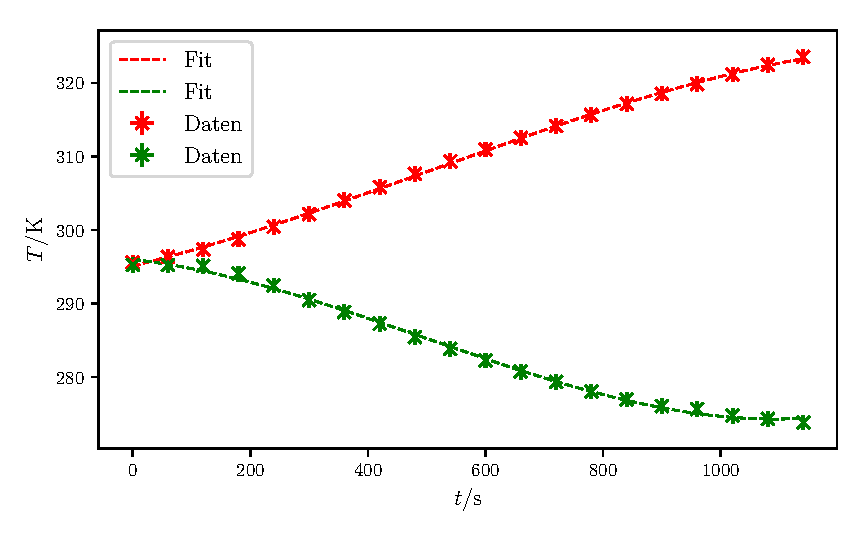
\includegraphics{build/plot1.pdf}
    \caption{Temperaturverläufe. Die rote Kurve stellt ... dar. Die grüne Kurve stellt ... dar.
    Die Fitparameter der Kurve der Temperatur im ersten Reservoir sind $A=\num{(-1.20 \pm 17.01)e-8}$,
    $B=\num{(1.83 \pm 29.53)e-5}$, $C=\num{(1.95 \pm 14.27)e-2}$ und $D=\SI{295.11 \pm 0.18}$.
    Die Fitparameter der Kurve der Temperatur im zweiten Reservoir sind $A=\num{}$,
    $B=\num{}$, $C=\num{}$ und $D=\num{}$.}
    \label{fig:plot1}
\end{figure}


\subsection{Bestimmung der Güteziffer}

\subsection{Bestimmung des Massendurchsatzes}

\subsection{Bestimmung der mechanischen Kompressorleistung}
\begin{align*}
    \rho_0 &= \SI{5.51}{\gram\per\liter} \\
    T &= \SI{273.15}{\kelvin} \\
    p &= \SI{e5}{\pascal} \\
    \kappa &= \num{1.14}
\end{align*}

